% 2011 年山东卷理科第 21 题：圆柱两端各接一个半球形的容器。
% 来源 PDF：普通高考/2011/2011山东理.pdf，SHA-256 d0f409fd3fa82b12c210d587c8412d4c446946a201f87d124e2fc17c5a50db16。
% 原页：第 2 页（A3 三栏）第 2 栏中部，书页码 690。
% 重绘依据：照原页——中间圆柱（长 l，半径 r），左右两端各为半径 r 的半球；
%   两端各画一条竖直虚线（直径，上下各标 r）与一条水平虚线（半径，标 r）；
%   两端的交线圆画成椭圆：靠外的一半实线、靠里的一半虚线（照原页）；
%   顶部用双箭头标出圆柱长 l，箭头两端各有一条竖直短线。不按比例。
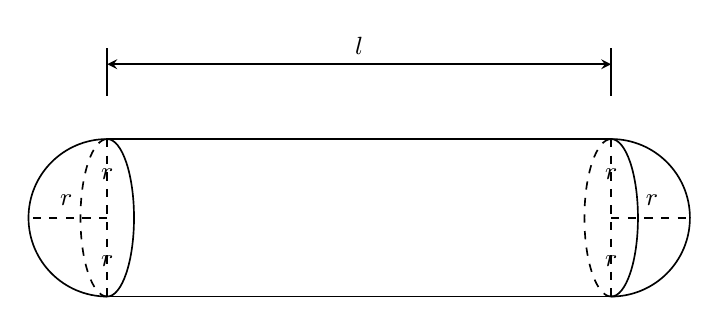
\begin{tikzpicture}[>=stealth, semithick, font=\small, x=1cm, y=1cm]
  \def\r{1.0}
  \def\L{6.4}
  \def\rx{0.34}
  % 圆柱母线
  \draw (0,\r) -- (\L,\r);
  \draw (0,-\r) -- (\L,-\r);
  % 两端半球的外轮廓
  \draw (0,\r) arc (90:270:\r);
  \draw (\L,-\r) arc (-90:90:\r);
  % 左端交线圆：左半实线、右半虚线
  \draw (0,\r) arc (90:-90:{\rx} and {\r});
  \draw[dashed] (0,-\r) arc (-90:-270:{\rx} and {\r});
  % 右端交线圆：左半实线、右半虚线
  \draw (\L,\r) arc (90:-90:{\rx} and {\r});
  \draw[dashed] (\L,-\r) arc (-90:-270:{\rx} and {\r});
  % 左端半径与直径
  \draw[dashed] (0,\r) -- (0,-\r);
  \draw[dashed] (0,0) -- (-\r,0);
  \node at (0,{0.55*\r}) {$r$};
  \node at (0,{-0.55*\r}) {$r$};
  \node at ({-0.52*\r},{0.22*\r}) {$r$};
  % 右端半径与直径
  \draw[dashed] (\L,\r) -- (\L,-\r);
  \draw[dashed] (\L,0) -- ({\L+\r},0);
  \node at (\L,{0.55*\r}) {$r$};
  \node at (\L,{-0.55*\r}) {$r$};
  \node at ({\L+0.52*\r},{0.22*\r}) {$r$};
  % 顶部标注 l
  \draw (\L,{\r+0.55}) -- (\L,{\r+1.15});
  \draw (0,{\r+0.55}) -- (0,{\r+1.15});
  \draw[<->] (0,{\r+0.95}) -- (\L,{\r+0.95});
  \node[above] at ({0.5*\L},{\r+0.95}) {$l$};
\end{tikzpicture}
